\subsection{Zadanie 2.1 Planowanie realizacji portfela przy ograniczonych kompetencjach}
\begin{figure}[htb]
\caption{Kompetencje zespołów}
\begin{center}
\begin{tabular}{ | c | c | c | c | c | c | c | }
\hline
  & A & B & C & D & E & F \\ 
 \hline
 1 & - & X & - & X & X & - \\  
 \hline
 2 & - & X & X & - & X & - \\
 \hline  
 3 & X & - & - & X & - & X \\
 \hline  
 4 & X & - & X & - & - & X \\
 \hline  
 5 & - & X & - & - & X & X \\
 \hline  
 6 & X & - & X & X & - & - \\
 \hline
\end{tabular}
\end{center}
\end{figure}
\subsubsection{Problem do rozwiązania}
\paragraph{Sformułowanie}
Matematyczne sformułowanie zadania:
\begin{enumerate}
\item Parametry \\
s - źródło \\
w - wyjście \\
N - węzły (N = {s, t, 1, 2, 3, 4, 5, 6, A, B, C, D, E, F})
P - projekty (P = {1, 2, 3, 4, 5, 6} $\subseteq$ N)
Z - zespoły (Z = {A, B, C, D, E, F} $\subseteq$ N)
$u_{ij}$ - przepustowość pomiędzy węzłem i a węzłem j
\item Zmienne decyzyjne
$f_{ij}$ - przepływ między węzłem i a węzłem j
\item Funkcja celu
\begin{align*}
    Q &= \max\left(\sum_{p \in P} f_{pt} \right) \\
    &= \max(f_{1t} + f_{2t} + f_{3t} + f_{4t} + f{5t} + f_{6t})
\end{align*}

\item Ograniczenia
\setcounter{equation}{0}
\begin{equation}
0 \leq f_{ij} \leq 1, (i, j) \in N
\end{equation}
\begin{equation}
0 \leq f_{zp} \leq u_{zp}, z \in Z, p \in P
\end{equation}
\begin{equation}
f_{si} = 0, i \in \{ s, t, 1, 2, 3, 4, 5, 6 \}
\end{equation}
\begin{equation}
f_{is} = 0, i \in N
\end{equation}
\begin{equation}
f_{ti} = 0, i \in N
\end{equation}
\begin{equation}
f_{it} = 0, i \in \{s, t, A, B, C, D, E, F\}
\end{equation}
\begin{equation}
\sum_{z \in Z} f_{zp} = 1, p \in P = \{ 1, 2, 3, 4, 5, 6 \}
\end{equation}

\begin{equation}
\sum_{p \in P} f_{zp} = 1, z \in Z = \{ A, B, C, D, E, F \}
\end{equation}

\begin{equation}
\sum_{i \in N \backslash \{s\}} f_{ni} = \sum_{j \in N \backslash \{t\}} f_{jn}, n \in N \backslash \{ s, t \}
\end{equation}



\end{enumerate}

\paragraph{Model sieciowy rysunek}
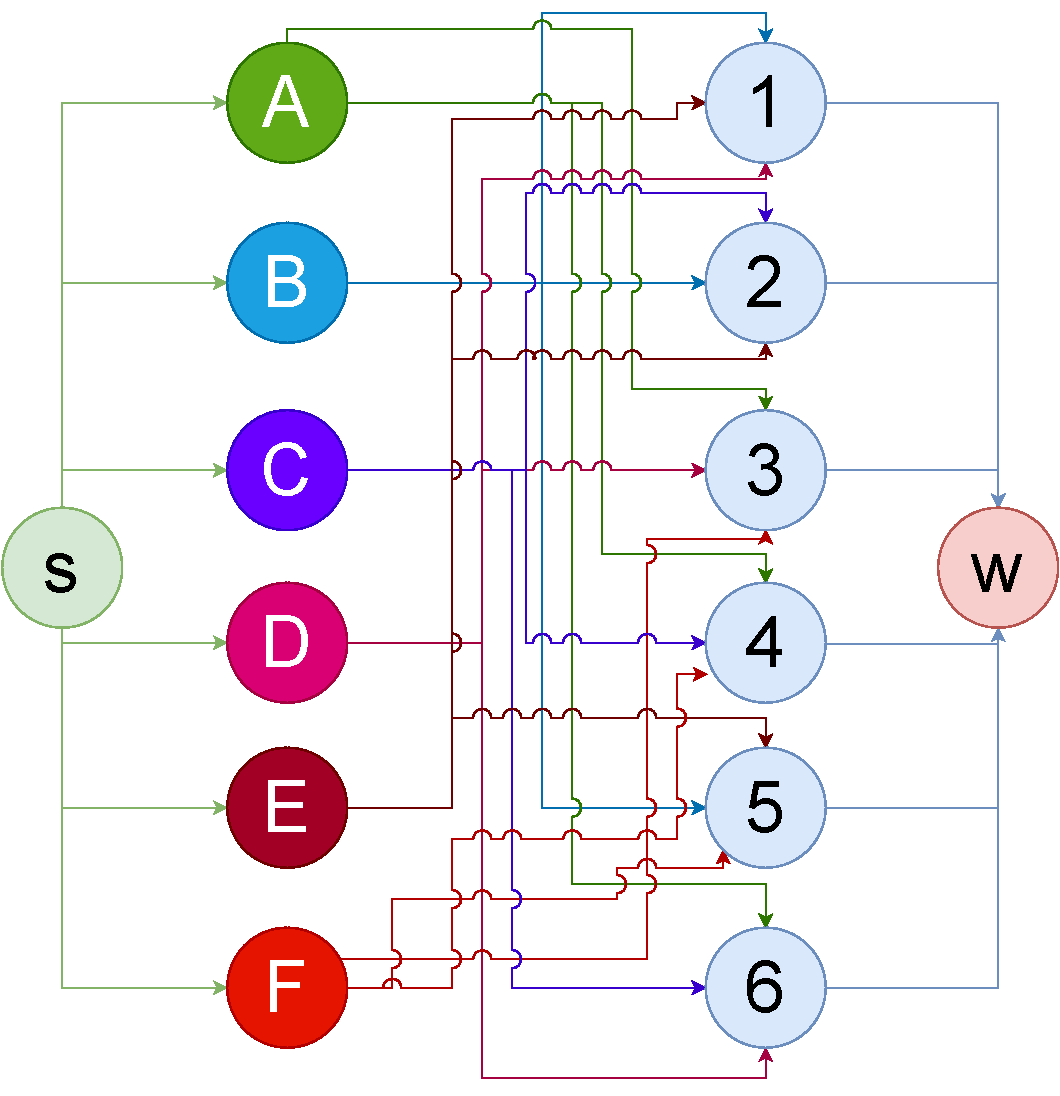
\includepdf[pages=-]{flowchart21.pdf}
\paragraph{Rozwiazanie}
\begin{lstlisting}[caption= plik dat]
data; 
 
set Wyjscie := t; 
set Wezly := 1, 2, 3, 4, 5, 6, A, B, C, D, E, F; 
set StartWezly := s, 1, 2, 3, 4, 5, 6, A, B, C, D, E, F; 
set WyjscieWezly := t, 1, 2, 3, 4, 5, 6, A, B, C, D, E, F; 
set StartWyjscieWezly := s, t, 1, 2, 3, 4, 5, 6, A, B, C, D, E, F; 
set Projekty := 1, 2, 3, 4, 5, 6; 
set Zespoly := A, B, C, D, E, F; 
 
param u := 
A 1 0 A 2 0 A 3 1 A 4 1 A 5 0 A 6 1
B 1 1 B 2 1 B 3 0 B 4 0 B 5 1 B 6 0 
C 1 1 C 2 0 C 3 1 C 4 0 C 5 0 C 6 1 
D 1 1 D 2 0 D 3 1 D 4 0 D 5 0 D 6 1 
E 1 1 E 2 1 E 3 0 E 4 0 E 5 1 E 6 0 
F 1 0 F 2 0 F 3 1 F 4 1 F 5 1 F 6 0; 
 
end; 
\end{lstlisting}
\begin{lstlisting}[caption= plik mod]
set Wyjscie; 
set Wezly; 
set StartWezly; 
set WyjscieWezly; 
set StartWyjscieWezly; 
set Projekty; 
set Zespoly; 
 
param u{z in Zespoly, p in Projekty}; 
 
var f{i in StartWyjscieWezly, j in StartWyjscieWezly}, >= 0; 
 
maximize Q: sum {p in Projekty, t in Wyjscie} f[p,t]; 
 
  Ograniczeni_jeden{i in StartWyjscieWezly, j in StartWyjscieWezly}: 
    f[i,j] >= 0; 
  Ograniczeni_dwa{i in StartWyjscieWezly, j in StartWyjscieWezly}: 
    f[i,j] <= 1; 
  Ograniczeni_trzy{p in Projekty, z in Zespoly}: 
    f[z,p] <= u[z,p]; 
  Ograniczeni_cztery{p in Projekty}: 
    sum {z in Zespoly} f[z,p] = 1; 
  Ograniczeni_piec{z in Zespoly}: 
    sum {p in Projekty} f[z,p] = 1; 
  Ograniczeni_szesc{n in Wezly}: 
    sum {i in WyjscieWezly} f[n,i] = sum {j in StartWezly} f[j,n]; 
	solve; 
display {i in Wezly, j in Wezly: f[i,j] > 0}: f[i,j]; 
display: Q;


\end{lstlisting}
\paragraph{Przydział zespołów do projektów}
\begin{lstlisting}[caption=wynik z glpk]
f[A,6].val = 1
f[B,5].val = 1
f[C,1].val = 1
f[D,3].val = 1
f[E,2].val = 1
f[F,4].val = 1
Q.val = 6
\end{lstlisting}
Wyniki: \\
Projekt numer \textbf{1} zostanie przydzielony zespołowi \textbf{C} \\
Projekt numer \textbf{2} zostanie przydzielony zespołowi \textbf{E} \\
Projekt numer \textbf{3} zostanie przydzielony zespołowi \textbf{D} \\
Projekt numer \textbf{4} zostanie przydzielony zespołowi \textbf{F} \\
Projekt numer \textbf{5} zostanie przydzielony zespołowi \textbf{B} \\
Projekt numer \textbf{6} zostanie przydzielony zespołowi \textbf{A} \\
